\chapter{Execução da Pesquisa}


\section{Ferramentas usadas}

O código será versionado no
Github\footnote{\url{https://github.com/diegofreitas/platform_packages_apps_contacts}}
onde será feito o gerenciamento das versões de cada iteração.
As ferramentas utilizadas para a refatoração serão a IDE Eclipse(Juno) com
plugin ADT v21 para facilitar a edição do código e ferramentas de construção
do projeto existentes no próprio repositório do android, tendo em vista que todo
o processo de compilação e empacotamento não visa ser usado em uma IDE.
Para realizar a coleta das métricas é necessário que a ferramenta analise código
java e contemple todas as métricas descritas na seção \ref{sec:metrics}. O
programa Chidamber and Kemerer Java
Metrics\footnote{\url{https://github.com/dspinellis/ckjm}} atende esses
critérios, além de ser um projeto de código-aberto.

\section{Análise do objeto de estudo}

O aplicativo a ser refatorado tem funcionalidades para gerenciamento de
contatos. Dentro deste conjunto de casos de uso será refatorado o pacote
referente ao gerenciamento de grupos de contatos presente no pacote
\textbf{com.android.contacts.group} que contém componentes de tela para
interação com o usuário, a saber:
\begin{description}
\item[GroupDetailFragment.java] Exibe os dados de um grupo de contatos.
\item[GroupBrowseListFragment.java] Fonece uma lista de grupos.
\item[GroupEditorFragment.java] Disponibiliza um formulário para edição dos
dados de um grupo.
\end{description}

Estas interfaces são usadas dentro de activities que controlam uma parte do fluxo
de interação e se comportam de forma diferente conforme o tipo de dispositivo
móvel utilizado. Devido a essa complexidade, não será feita nenhuma alteração na
interface pública dos componentes refatorados, evitando efeitos colaterais em
outras partes do aplicativo.

Os componentes elencados contêm código não somente relacionado com a lógica de
apresentação como também interagem diretamente com classes destinadas ao acesso
de dados e serviços existentes nas dependências do projeto, por exemplo,
gerenciamento de contas do usuário. 

Cada iteração consistirá na refatoração de cada um dos componentes
descritos. O marco de referência de dados das métricas presentes na tabela \ref{tab:dados_baseline} será feita a partir da
versão \verb|4.4.2_r1| do aplicativo.

\begin{table}[h]
	\centering
    \begin{tabular}{ | l | l | }
    \hline
    Métrica &	Média \\ \hline
    WMC  	&	8.5161290323   	\\ \hline
    DIT	 	&	0.7741935484	\\ \hline
	NOC  	& 	0				\\ \hline
	CBO	  	& 	10.1612903226	\\ \hline
	RFC	 	& 	23.7419354839	\\ \hline
	LCOM 	& 	57.4838709677	\\ \hline
    \end{tabular}
    \caption{Métricas CK da versão de referência}
    \label{tab:dados_baseline}
\end{table}

\section{Arquitetura Proposta}

% sempre que for referenciar as camadas (view, model, controller), utilize com primeira maiúscula. serve tb para nome de classes e padroes citados ao longo do texto

Será aplicado nos experimentos a variação do padrão MVP chamada Passive View,
pois dessa forma, o Model não precisa publicar alterações de seu estado para a
view, Logo, evita-se alterações no código referente às classes que fazem
parte da camada de Model do aplicativo de contatos. A organização do código
fonte no repositório dificulta a implementação, isto porque esses componentes estão
localizados fora do projeto afetado e são compartilhados.

As classes que extendem Fragment terão a responsabilidade da View, pois é neste
componente que a interface com o usuário é construída. A classe Activity fornece
vários métodos para recuperação de recursos de imagens, textos, inicialização de
serviços, entre outros. Isso ocorre porque a classe Activity é uma subclasse de Context, herdando diversos métodos não relacionados ao gerenciamento da interface.

Segundo \citeonline{Reenskaug:1979} ``\ldots Os papéis da View e do
Controller podem ser exercidos pelo mesmo objeto quando eles estão muito
acoplados. Exemplo: Um Menu.''(tradução livre). Porém, isso requer um boa
análise do problema em questão para decidir o nível de granularidade que esses componentes podem ter.
Portanto, é recomendável manter sempre essa separação para manter uma boa coesão
nas classes. O Presenter será uma classe auxiliar à view e pode ser implementada
como uma classe java simples. 



\section{Resultados dos Experimentos}

Esta sessão tem como objetvo mostar os resultados objetos com o processo de
refatoração aplicando o parão mvp. Cada métrica é apresentada com seus dados
para cada iteração mostrando os efeitos desses valores na qualidade.

\subsection{WMC}


A métrica WMC é usada para medir o tempo e esforço necessário para desenvolver e
manter uma classe. É recomendado que esta métrica tenha valores baixos. A
tablela \ref{tab:wmc} e a figura \ref{fig:wmc} mostram os valores dessa métricas
no projeto.

Segundo \citeonline{cksuite} “\ldots Classes com um número grande de métodos
tem uma aplicação específica limitando a possibilidade de reuso."(tradução
livre). As classes que foram refatoradas são de interface, portanto
implementam uma interação com o usuário bem específica que não serão
reutilizadas por meio de herança.
\begin{table}[h]
	\centering
    \begin{tabular}{ | l | l | }
    \hline
    Iteração & Média 			\\ \hline
    Baseline & 8.5161290323   	\\ \hline
    Iteração 1 & 8.875			\\ \hline
	Iteração 2 & 9				\\ \hline
	Iteração 3 & 8.9393939394	\\ \hline
    \end{tabular}
    \caption{Dados métrica WMC}
    \label{tab:wmc}
\end{table}

\begin{figure}[h]
	\centering
	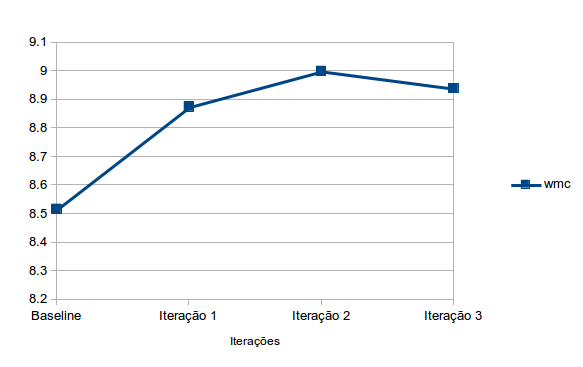
\includegraphics{img/wmc.png}
	\caption{Gráfico da métrica WMC/Fonte: Próprio autor} 
	\label{fig:wmc}
\end{figure}


\subsection{DIT}

A métrica DIT esta relacionado complexidade e reusabilidade. Quanto mais abaixo
na hierarquia de heraça a classe estiver, menos previsível será seu
comportamento devido a quantidade de classes acima. Entretanto, a métrica também
indica um potencial reuso de código por meio da herança de métodos, isso torna
os parâmetros de avaliação da métrica dependentes do contexto a ser analisado.
O aumento demonstrado na DIT se deve ao fato que o ckjm considera a
implementação de interface como herança. A interface define somente o contrato
que a classe de implementar não havendo nenhuma implementação que pudesse
interferir no comportamento da classe, portanto essa alteração no DIT não deve
ser considerada. O aumento no valor da métrica é mostrado na
tabela~\ref{tab:dit} e Figura~\ref{fig:dit}

\begin{table}[h]
	\centering
    \begin{tabular}{ | l | l | }
    \hline
    Iteração & Média 			\\ \hline
    Baseline & 0.7741935484  	\\ \hline
    Iteração 1 & 0.78125		\\ \hline
	Iteração 2 & 0.78125			\\ \hline
	Iteração 3 & 0.7878787879	\\ \hline
    \end{tabular}
    \caption{Dados métrica DIT}
    \label{tab:dit}
\end{table}

\begin{figure}[h]
	\centering
	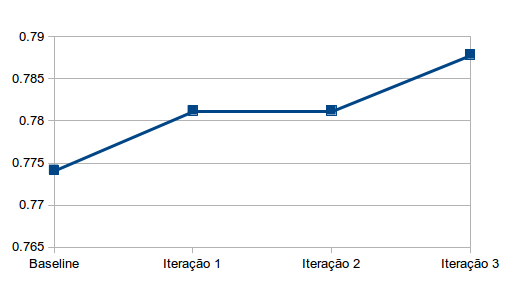
\includegraphics{img/dit.png}
	\caption{Valores de DIT/Fonte: Próprio autor}
	\label{fig:dit}
\end{figure}


\subsection{NOC}

Altos valores para a métrica NOC são indicativos de que existe maior reuso de
código, o esforço de testes também aumenta e maior é a probabilidade de uso
incorreto de abstração. O objetivo da métrica é variável Nenhuma classe foi
herdada para a aplicação do padrão, portanto, essa métrica permaneceu intacta
durante as iterações como pode ser observado na tabela \ref{tab:noc} e
figura~\ref{fig:noc}

\begin{table}[h]
	\centering
    \begin{tabular}{ | l | l | }
    \hline
    Iteração & Média 			\\ \hline
    Baseline & 0  	\\ \hline
    Iteração 1 & 0			\\ \hline
	Iteração 2 & 0				\\ \hline
	Iteração 3 & 0	\\ \hline
    \end{tabular}
    \caption{Dados métrica NOC}
    \label{tab:noc}
\end{table}

\begin{figure}[h]
	\centering
	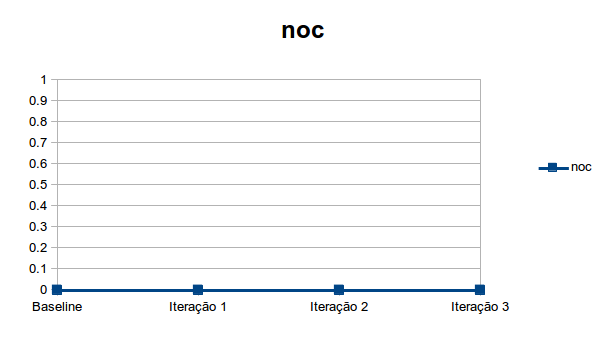
\includegraphics{img/noc.png}
	\caption{Valores de NOC/Fonte: Próprio autor}
	\label{fig:noc}
\end{figure}

\subsection{CBO}

Valores baixos de CBO são indicativos de boa modularidade e encapsulamento que
se reflete na indepdendência da classe o que a torna mais fácil de reutilizar,
manter e testar.

Na primeira iteração foi aplicado o padrão em um componente mais simples e foi
possível remover qualquer dependência que não fosse relacionada a interface,
entretanto, a maior queda ocorreu em  ficando a cargo do da experiência do
desenvolvedor identificar estes cenários específicos. Nas iterações seguintes as
interfaces alteradas são mais complexos,

\begin{table}[h]
	\centering
    \begin{tabular}{ | l | l | }
    \hline
    Iteração & Média 			\\ \hline
    Baseline & 10.1612903226   	\\ \hline
    Iteração 1 & 10.03125		\\ \hline
	Iteração 2 & 10.09375		\\ \hline
	Iteração 3 & 10.1515151515	\\ \hline
    \end{tabular}
    \caption{Dados métrica CBO}
    \label{tab:cbo}
\end{table}

\begin{figure}[h]
	\centering
	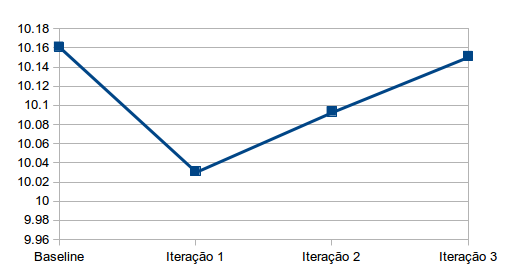
\includegraphics{img/cbo.png}
	\caption{Valores de CBO/Fonte: Próprio autor}
	\label{fig:cbo}
\end{figure}


\subsection{RFC}

Altos valores para a métrica RFC indica que uma quantidade grande de métodos é
chamados a partir de uma classe tornando-a mais complexa de testar e fazer
manutenção. Logo, esta métrica deve ser mantida baixa.

A métrica RFC tende a aumentar a cada iteração o que sugere um aumento da
complexidade do código conforme é apresentado na tabela \ref{tab:rfc} e Figura
\ref{fig:rfc}.

\begin{table}[h]
	\centering
    \begin{tabular}{ | l | l | }
    \hline
    Iteração & Média 			\\ \hline
    Baseline & 23.7419354839   	\\ \hline
    Iteração 1 & 24.21875		\\ \hline
	Iteração 2 & 24.71875		\\ \hline
	Iteração 3 & 24.9090909091	\\ \hline
    \end{tabular}
    \caption{Dados métrica RFC}
    \label{tab:rfc}
\end{table}

\begin{figure}[h]
	\centering
	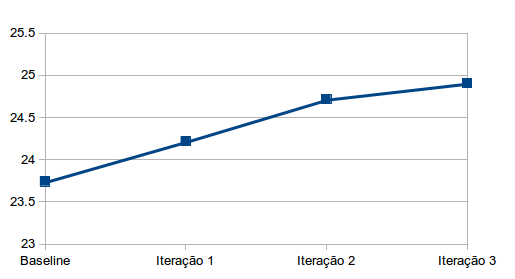
\includegraphics{img/rfc.png}
	\caption{Valores de RFC/Fonte: Próprio autor}
	\label{fig:rfc}
\end{figure}

\subsection{LCOM}

Esta métrica ajuda a identificar má qualidade na estrutura do código quando os
valores são altos apontando aumento da complexidade e pouco encapsulamento.
A tabela \ref{tab:lcom} e a figura \ref{fig:lcom} mostram uma queda
siginificativa na métrica LCOM.
Isto indica que a coesão do código melhorou após cada iteração. 

\begin{table}[h]
	\centering
    \begin{tabular}{ | l | l | }
    \hline
    Iteração & Média 			\\ \hline
    Baseline & 57.4838709677   	\\ \hline
    Iteração 1 & 56.875			\\ \hline
	Iteração 2 & 53.1875		\\ \hline
	Iteração 3 & 48.4242424242	\\ \hline
    \end{tabular}
    \caption{Dados métrica LCOM}
    \label{tab:lcom}
\end{table}

\begin{figure}[h]
	\centering
	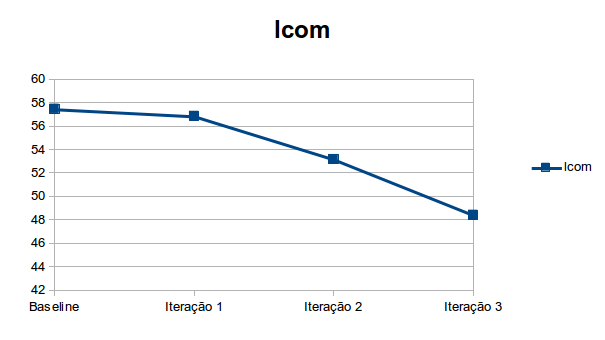
\includegraphics{img/lcom.png}
	\caption{Valores de lcom/Fonte: Próprio autor}
	\label{fig:lcom}
\end{figure}
